%iffalse
\let\negmedspace\undefined
\let\negthickspace\undefined
\documentclass[journal,12pt,onecolumn]{IEEEtran}
\usepackage{cite}
\usepackage{amsmath,amssymb,amsfonts,amsthm}
\usepackage{algorithmic}
\usepackage{graphicx}
\usepackage{textcomp}
\usepackage{xcolor}
\usepackage{txfonts}
\usepackage{listings}
\usepackage{enumitem}
\usepackage{mathtools}
\usepackage{gensymb}
\usepackage{comment}
\usepackage[breaklinks=true]{hyperref}
\usepackage{tkz-euclide} 
\usepackage{listings}
\usepackage{gvv}
\usepackage[latin1]{inputenc}
\usepackage{color}
\usepackage{array}
\usepackage{longtable}
\usepackage{calc}
\usepackage{multirow}
\usepackage{hhline}
\usepackage{ifthen}
\usepackage{lscape}
\usepackage{tabularx}
\usepackage{array}
\usepackage{float}
\usepackage{multicol}
\usepackage{subcaption}

\newtheorem{theorem}{Theorem}[section]
\newtheorem{problem}{Problem}
\newtheorem{proposition}{Proposition}[section]
\newtheorem{lemma}{Lemma}[section]
\newtheorem{corollary}[theorem]{Corollary}
\newtheorem{example}{Example}[section]
\newtheorem{definition}[problem]{Definition}
\newcommand{\BEQA}{\begin{eqnarray}}
\newcommand{\EEQA}{\end{eqnarray}}
\newcommand{\define}{\stackrel{\triangle}{=}}
\theoremstyle{remark}
\newtheorem{rem}{Remark}

% Marks the beginning of the document
\begin{document}
\bibliographystyle{IEEEtran}
\vspace{3cm}

\title{2024-AE-'40-52'}
\author{S.Sai Akshitha - EE24BTECH11054}
\newpage
\maketitle
\bigskip

\renewcommand{\thefigure}{\theenumi}
\renewcommand{\thetable}{\theenumi}

\begin{enumerate}
    \item A multistage axial compressor, with overall isentropic efficiency of 0.83, is used to compress air at a stagnation temperature of 300 K through a pressure ratio of 10:1. Each stage of the compressor is similar, and the stagnation temperature rise across each compressor stage is 20 K. Assume $C_p$=1005 J/kg K and $\gamma=$1.4 for air. How many stages are there in the compressor?
    
    \begin{enumerate}
        \item 17
        \item 13
        \item 19
        \item 11
    \end{enumerate}
    
    \item An aircraft with a turbojet engine is flying at 250 m/s. The uninstalled thrust produced by the engine is 60000 N. The heating value of the fuel is $44 \times 10^6$ J/kg. The engine has a thermal efficiency of 35% while burning the fuel at a rate of 3 kg/s. Assume the engine exit pressure to be equal to the ambient pressure. What is the propulsion efficiency of the engine under these conditions (in percentage)?
    
    \begin{enumerate}
        \item 32.5
        \item 35.0
        \item 11.4
        \item 92.4
    \end{enumerate}
    
    \item Consider a flat plate, with a sharp leading edge, placed in a uniform flow of speed $U$. The direction of the free-stream flow is aligned with the plate. Assume that the flow is steady, incompressible and laminar. The thickness of the boundary layer at a fixed stream-wise location $L$ from the leading edge of the plate is $\delta$. Which one of the following correctly describes the variation of $\delta$ with $U$?
    
    \begin{enumerate}
        \item $\delta \propto U$
        \item $\delta \propto {U}^{\frac{3}{2}}$
        \item $\delta \propto {U}^{\frac{1}{2}}$
        \item $\delta \propto {U}^{\frac{-1}{2}}$
    \end{enumerate}
    
    \item Shock structures for flow at three different Mach numbers over a given wedge are shown in the figure below. Assuming that only the weak shock solutions are possible for the attached oblique shocks, which one of the following options is TRUE?
    
    \begin{figure}[H]
        \centering
        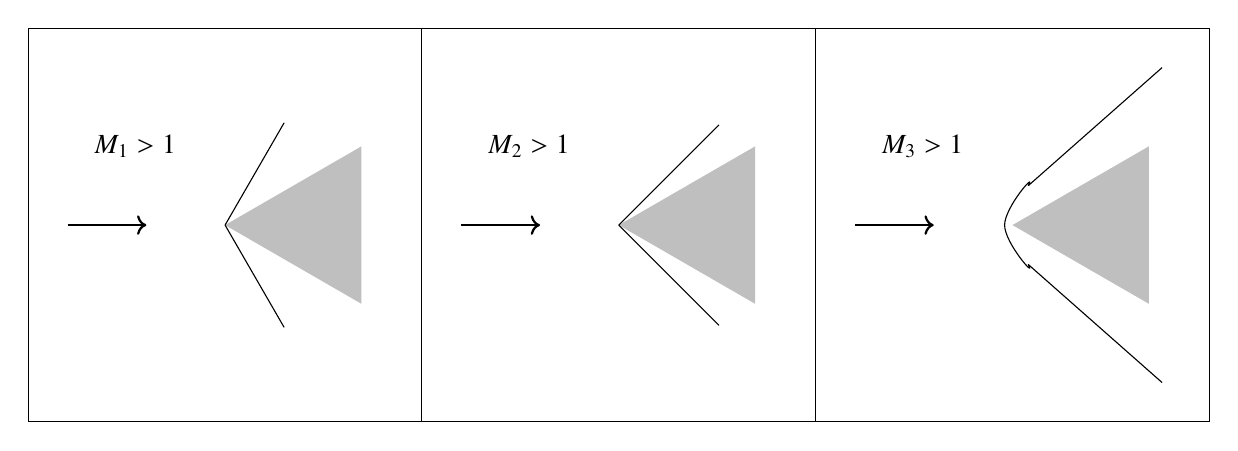
\begin{tikzpicture}
    % Draw the outer rectangle
    \draw (0,0) rectangle (15,5);
    
    % Split the rectangle into three parts
    \draw (5,0) -- (5,5);
    \draw (10,0) -- (10,5);
    
    % First panel: left
    \node[left] at (2.0,3.5) {$M_1 > 1$};
    \draw[->, thick] (0.5,2.5) -- (1.5,2.5);
    \fill[gray!50] (2.5,2.5) -- ++(30:2) -- ++(-90:2) -- cycle;
    \draw (2.5,2.5) -- ++(60:1.5);
    \draw (2.5,2.5) -- ++(-60:1.5);

    % Second panel: middle
    \node[left] at (7.0,3.5) {$M_2 > 1$};
    \draw[->, thick] (5.5,2.5) -- (6.5,2.5);
    \fill[gray!50] (7.5,2.5) -- ++(30:2) -- ++(-90:2) -- cycle;
    \draw (7.5,2.5) -- ++(45:1.8);
    \draw (7.5,2.5) -- ++(-45:1.8);

    % Third panel: right
    \node[left] at (12.0,3.5) {$M_3 > 1$};
    \draw[->, thick] (10.5,2.5) -- (11.5,2.5);
    \fill[gray!50] (12.5,2.5) -- ++(30:2) -- ++(-90:2) -- cycle;
    \draw (12.4,2.5) to[out=+90,in=60] ++(0.3,0.5);
    \draw (12.4,2.5) to[out=-90,in=-60] ++(0.3,-0.5);
    \draw (12.7,3) -- (14.4,4.5);
    \draw (12.7,2) -- (14.4,0.5);
\end{tikzpicture}  
    \end{figure}
    
    \begin{enumerate}
        \item $M_1<M_2<M_3$
        \item $M_1>M_2>M_3$
        \item $M_1<M_3<M_2$
        \item $M_3<M_1<M_2$
    \end{enumerate}
    
    \item Air flowing at Mach number $M = 2$ from left to right accelerates to $M = 3$ across an expansion corner as shown in the figure. What is the value of $\delta$ (the angle between the Forward and Rearward Mach lines) in degrees? \\ The values of the Prandtl-Meyer functions are $v(3)=49.76 \degree$ and $v(2)=26.38\degree$
    
    \begin{figure}[H]
        \centering
        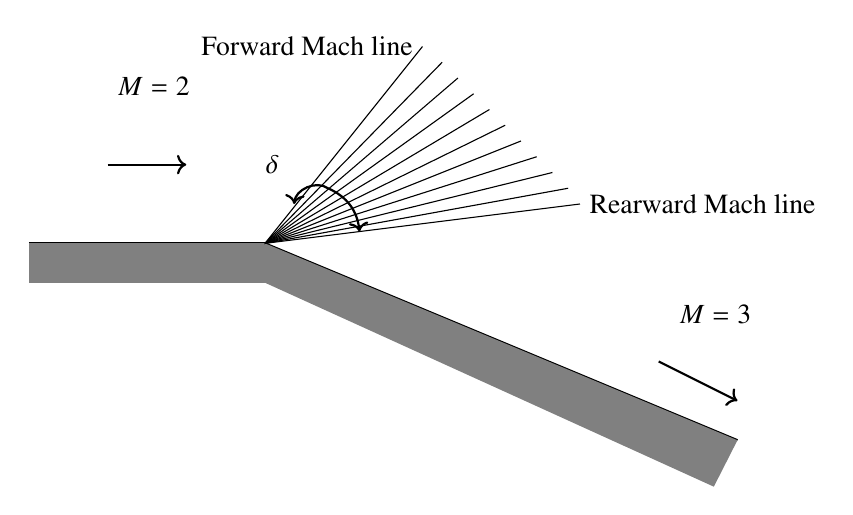
\begin{tikzpicture}
    


    \draw[thick] (-1,5.5) -- (2,5.5);
    \fill[gray!] (-1,5) -- (-1,5.5) -- (2,5.5) -- (2,5) -- cycle;
    \draw[thick] (2,5.5) -- (8,3);
    \fill[gray!] (2,5.5) -- (8,3) -- (7.7,2.41) -- (2,5) -- cycle;
    % Add other related components or labels as needed
    \node[right] at (0,7.5) {$M=2$};
    \draw[->, thick] (0,6.5) -- (1,6.5);

    \draw (2,5.5) -- (4,8)  node[left] {Forward Mach line};
    \draw (2,5.5) -- (6,6)  node[right] {Rearward Mach line};
    \draw (2,5.5) -- (5.85,6.2) ;
    \draw (2,5.5) -- (5.65,6.4) ;
\draw (2,5.5) -- (5.45,6.6) ;
\draw (2,5.5) -- (5.25,6.8) ;
\draw (2,5.5) -- (5.05,7) ;
\draw (2,5.5) -- (4.85,7.2) ;
\draw (2,5.5) -- (4.65,7.4) ;
\draw (2,5.5) -- (4.45,7.6) ;
\draw (2,5.5) -- (4.25,7.8) ;


 \draw[<->, thick] (2.37,6.0) to[bend left=60] (2.8,6.2) to[bend left=30] (3.2,5.65);


    \node[left] at (8.3,4.6) {$M=3$};
    \node[left] at (2.3,6.5) {$\delta$};
     \draw[->, thick] (7,4) -- (8,3.5);
\end{tikzpicture}
    \end{figure}
    
    \begin{enumerate}
        \item 23.38
        \item 19.47
        \item 53.38
        \item 33.91
    \end{enumerate}
    
    \item Consider the function 
    \[
    f(x)= 
    \begin{cases} 
        x^2 & x<0 \\
        x & x \geq 0 
    \end{cases}
    \]
    where $x$ is real. Which of the following statements is/are correct?
    
    \begin{enumerate}
        \item The function is continuous for all $x$
        \item The derivative of the function is discontinuous at $x = 0$
        \item The derivative of the function is continuous at $x = 1$
        \item The function is discontinuous at $x = 0$
    \end{enumerate}
    
    \item The figure shows plots of two yield loci for an isotropic material, where $\sigma_I$ and $\sigma_{II}$ are the principal stresses and $\sigma_Y$ is the yield stress in uniaxial tension. Which of the following statements is/are correct?
    
    \begin{figure}[H]
        \centering
        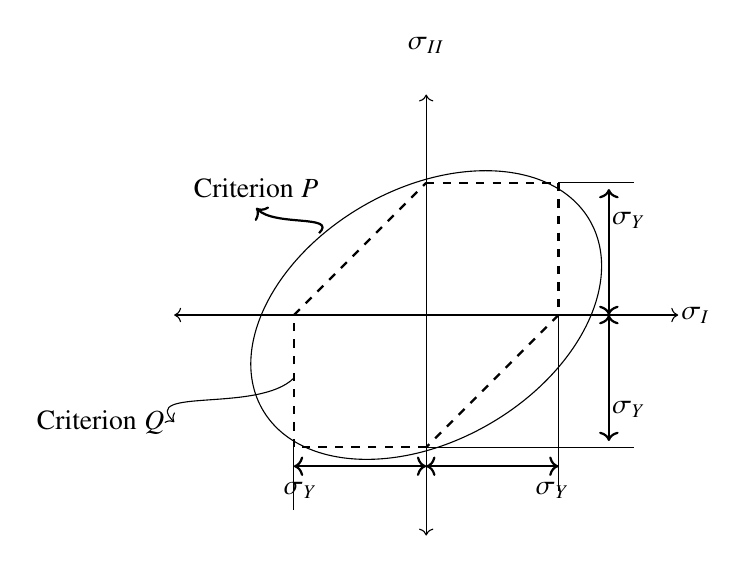
\begin{tikzpicture}[scale=0.8]
\draw[<->] (-4,0) -- (4,0);
\draw[<->] (0,-3.5) -- (0,3.5);
\draw[thick, dashed] (0,2.1) -- (2.1,2.1);
\draw[thick, dashed] (2.1,2.1) -- (2.1,0);
\draw[thick, dashed] (2.1,0) -- (0,-2.1);
\draw[thick, dashed] (0,-2.1) -- (-2.1,-2.1);
\draw[thick, dashed] (-2.1,-2.1) -- (-2.1,0);
\draw[thick, dashed] (-2.1,0) -- (0,2.1);
\draw[rotate=30] (0,0) ellipse (3cm and 2cm);
\draw (2.1,2.1) -- (3.3,2.1);
\draw (0,-2.1) -- (3.3,-2.1);
\draw (2.1,0) -- (2.1,-2.8);
\draw (-2.1,-2.1) -- (-2.1,-3.1);

\node[above] at (0,4) {$\sigma_{II}$};
\node[right] at (3.9,0) {$\sigma_I$};
\draw[<->][thick] (2.9,-2) -- (2.9,0);
\draw[<->][thick] (2.9,0) -- (2.9,2);
\node[right] at (2.8,1.5) {$\sigma_Y$};
\draw[<->][thick] (2.1,-2.4) -- (0,-2.4);
\draw[<->][thick] (0,-2.4) -- (-2.1,-2.4);
\node[below] at (-2,-2.5) {$\sigma_Y$};
\node[below] at (2,-2.5) {$\sigma_Y$};
\node[right] at (2.8,-1.5) {$\sigma_Y$};
\draw[->][thick] (-1.7,1.3) to [out=45,in=315] (-2.7,1.7);
\node[above] at (-2.7,1.7) {Criterion $P$};
\draw[->] (-2.1,-1) to [out=225,in=135] (-4,-1.7);
\node[left] at (-4,-1.7) {Criterion $Q$};
\end{tikzpicture}
    \end{figure}
    
    \begin{enumerate}
        \item Criterion $P$ represents the von Mises criterion
        \item Criterion $Q$ represents the Tresca criterion
        \item Criterion $P$ represents the Tresca criterion
        \item Criterion $Q$ represents the von Mises criterion
    \end{enumerate}
    
    \item Which of the following statements about absolute ceiling and service ceiling for a piston-propeller aircraft is/are correct?
    
    \begin{enumerate}
        \item The altitude corresponding to absolute ceiling is higher than that for service ceiling
        \item At the absolute ceiling, the power required for cruise equals the maximum power available
        \item The altitude corresponding to absolute ceiling is lower than that for service ceiling
        \item At the service ceiling, the maximum rate of climb is 50 ft/min
    \end{enumerate}
    
    \item For an airplane having directional/weathercock static stability, which of the following options is/are correct?
    
    \begin{enumerate}
        \item The airplane when disturbed in yaw, from an equilibrium state, will experience a restoring moment
        \item The variation of yawing moment coefficient $(C_n)$ with sideslip angle $(\beta)$ for the airplane will look like:
        
        \begin{figure}[H]
            \centering
            \begin{tikzpicture}

   \draw[thick,->] (4.5,4.5) -- (9,4.5) node[anchor=north west] {$\beta(+)$};
\draw[thick,->] (4.5,4.5) -- (4.5,9) node[anchor=south west] {$C_n(+)$};
\draw[thick,->] (4.5,4.5) -- (0,4.5)  node[anchor=north west] {$\beta(-)$};
\draw[thick,->] (4.5,4.5) -- (4.5,0) node[anchor=south west] {$C_n(-)$};
\draw (1,1) -- (8,8) ;
    
\end{tikzpicture}
        \end{figure}
        
        \item The airplane will always tend to point into the relative wind
        \item The airplane when disturbed in yaw will return to equilibrium state in a finite amount of time after removing the disturbance
    \end{enumerate}
    
    \item Which of the following statements is/are TRUE for an axial turbine?
    
    \begin{enumerate}
        \item For a fixed rotational speed, the mass flow rate increases with increase in the flow coefficient
        \item The absolute stagnation enthalpy of the flow decreases across the nozzle row
        \item The relative stagnation enthalpy remains unchanged through the rotor
        \item For a fixed rotational speed, the mass flow rate remains unchanged with a change in the flow coefficient
    \end{enumerate}
    
    \item Which of the following statements is/are TRUE for a single stage axial compressor?
    
    \begin{enumerate}
        \item Starting from design condition and keeping the mass flow rate constant, if the blade RPM is increased, the compressor rotor may experience positive incidence flow separation (actual relative flow angle greater than the design blade angle)
        \item Starting from design condition at the same blade RPM, if the mass flow rate is increased, the compressor rotor may experience positive incidence flow separation (actual relative flow angle greater than the design blade angle)
        \item Keeping the mass flow rate constant, if the blade RPM is increased, the compressor may experience surge
        \item At the same blade RPM, if the mass flow rate is increased, the compressor may experience surge
    \end{enumerate}
    
    \item Consider the matrix 
    $
    A = \myvec{ 5 & -4 }\\ \myvec{k & -1} ,
    $
    where $k$ is a constant. If the determinant of $A$ is 3, then the ratio of the largest eigenvalue of $A$ to the constant $k$ is $\rule{3cm}{0.15mm}$ (rounded off to 1 decimal place).
    
    \item The state of stress at a point is caused by two separate loading cases. One of them produces a pure uniaxial tension along the $x'$ direction, and the other one produces a pure uniaxial compression along the $y'$ direction, as shown in the figure. The sum of maximum and minimum principal stresses for the resultant state of stress caused by both loads acting simultaneously is $\rule{3cm}{0.15mm}$ N/mm$^2$ (rounded off to 1 decimal place).
    
    \begin{figure}[H]
        \centering
        
    % First subfigure
    \begin{subfigure}[b]{0.45\textwidth}
        \centering
        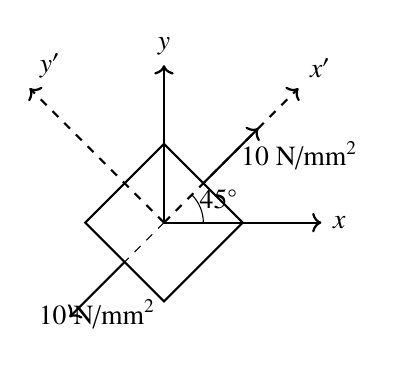
\begin{tikzpicture}
        \draw [thick,->] (0,0) -- (2,0) node[right] {$x$};
\draw [thick,->] (0,0) -- (0,2) node[above] {$y$};
\draw [thick,->,dashed] (0,0) -- (1.707,1.707) node[above right] {$x'$};
\draw [thick,->,dashed] (0,0) -- (-1.707,1.707) node[above right] {$y'$}; 
\draw [thick] (0,1) -- (1,0) -- (0,-1) -- (-1,0) -- cycle;
\draw [thick,->] (0.5,0.5) -- (1.2,1.2) node[midway,right] {$10 \text{ N/mm}^2$};
\draw [thick,->] (-0.5,-0.5) -- (-1.2,-1.2) node[midway,below] {$10 \text{ N/mm}^2$};
\draw [dashed] (0,0) -- (-0.5,-0.5);
\draw (0.5,0) arc (0:45:0.5) ;
\node at (0.7,0.3) {$45^\circ$};

            
        \end{tikzpicture}
        \caption{State of stress in case I}
        
    \end{subfigure}
    \hfill
    % Second subfigure
    \begin{subfigure}[b]{0.45\textwidth}
        \centering
        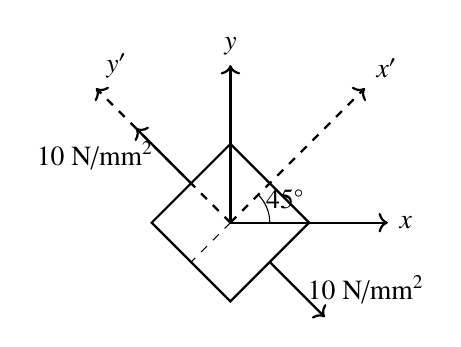
\begin{tikzpicture}
\draw [thick,->] (0,0) -- (2,0) node[right] {$x$};
\draw [thick,->] (0,0) -- (0,2) node[above] {$y$};
\draw [thick,->,dashed] (0,0) -- (1.707,1.707) node[above right] {$x'$};
\draw [thick,->,dashed] (0,0) -- (-1.707,1.707) node[above right] {$y'$}; 
\draw [thick] (0,1) -- (1,0) -- (0,-1) -- (-1,0) -- cycle;
\draw [thick,->] (0.5,-0.5) -- (1.2,-1.2) node[midway,right] {$10 \text{ N/mm}^2$};
\draw [thick,->] (-0.5,0.5) -- (-1.2,1.2) node[midway,left] {$10 \text{ N/mm}^2$};
\draw [dashed] (0,0) -- (-0.5,-0.5);
\draw (0.5,0) arc (0:45:0.5) ;
\node at (0.7,0.3) {$45^\circ$};

        \end{tikzpicture}
        \caption{State of stress in case II}
    \end{subfigure}
    \label{fig:tikz_subfigures}


    \end{figure}
    
\end{enumerate}

\end{document}

